\documentclass[journal,12pt,twocolumn]{IEEEtran}

\usepackage{setspace}
\usepackage{gensymb}
\singlespacing
\usepackage[cmex10]{amsmath}

\usepackage{amsthm}

\usepackage{mathrsfs}
\usepackage{txfonts}
\usepackage{stfloats}
\usepackage{bm}
\usepackage{cite}
\usepackage{cases}
\usepackage{subfig}

\usepackage{longtable}
\usepackage{multirow}

\usepackage{enumitem}
\usepackage{mathtools}
\usepackage{steinmetz}
\usepackage{tikz}
\usepackage{circuitikz}
\usepackage{verbatim}
\usepackage{tfrupee}
\usepackage[breaklinks=true]{hyperref}
\usepackage{graphicx}
\usepackage{tkz-euclide}

\usetikzlibrary{calc,math}
\usepackage{listings}
    \usepackage{color}                                            %%
    \usepackage{array}                                            %%
    \usepackage{longtable}                                        %%
    \usepackage{calc}                                             %%
    \usepackage{multirow}                                         %%
    \usepackage{hhline}                                           %%
    \usepackage{ifthen}                                           %%
    \usepackage{lscape}     
\usepackage{multicol}
\usepackage{chngcntr}

\DeclareMathOperator*{\Res}{Res}

\renewcommand\thesection{\arabic{section}}
\renewcommand\thesubsection{\thesection.\arabic{subsection}}
\renewcommand\thesubsubsection{\thesubsection.\arabic{subsubsection}}

\renewcommand\thesectiondis{\arabic{section}}
\renewcommand\thesubsectiondis{\thesectiondis.\arabic{subsection}}
\renewcommand\thesubsubsectiondis{\thesubsectiondis.\arabic{subsubsection}}


\hyphenation{op-tical net-works semi-conduc-tor}
\def\inputGnumericTable{}                                 %%

\lstset{
%language=C,
frame=single, 
breaklines=true,
columns=fullflexible
}
\begin{document}

\newcommand{\BEQA}{\begin{eqnarray}}
\newcommand{\EEQA}{\end{eqnarray}}
\newcommand{\define}{\stackrel{\triangle}{=}}
\bibliographystyle{IEEEtran}
\raggedbottom
\setlength{\parindent}{0pt}
\providecommand{\mbf}{\mathbf}
\providecommand{\pr}[1]{\ensuremath{\Pr\left(#1\right)}}\newcommand*{\permcomb}[4][0mu]{{{}^{#3}\mkern#1#2_{#4}}}
\newcommand*{\perm}[1][-3mu]{\permcomb[#1]{P}}
\newcommand*{\comb}[1][-1mu]{\permcomb[#1]{C}}
\providecommand{\qfunc}[1]{\ensuremath{Q\left(#1\right)}}
\providecommand{\sbrak}[1]{\ensuremath{{}\left[#1\right]}}
\providecommand{\lsbrak}[1]{\ensuremath{{}\left[#1\right.}}
\providecommand{\rsbrak}[1]{\ensuremath{{}\left.#1\right]}}
\providecommand{\brak}[1]{\ensuremath{\left(#1\right)}}
\providecommand{\lbrak}[1]{\ensuremath{\left(#1\right.}}
\providecommand{\rbrak}[1]{\ensuremath{\left.#1\right)}}
\providecommand{\cbrak}[1]{\ensuremath{\left\{#1\right\}}}
\providecommand{\lcbrak}[1]{\ensuremath{\left\{#1\right.}}
\providecommand{\rcbrak}[1]{\ensuremath{\left.#1\right\}}}
\theoremstyle{remark}
\newtheorem{rem}{Remark}
\newcommand{\sgn}{\mathop{\mathrm{sgn}}}
\providecommand{\abs}[1]{\vert#1\vert}
\providecommand{\res}[1]{\Res\displaylimits_{#1}} 
\providecommand{\norm}[1]{\lVert#1\rVert}
\providecommand{\pr}[1]{\ensuremath{\Pr\left(#1\right)}}
%\providecommand{\norm}[1]{\lVert#1\rVert}
\providecommand{\mtx}[1]{\mathbf{#1}}
\providecommand{\mean}[1]{E[ #1 ]}
\providecommand{\fourier}{\overset{\mathcal{F}}{ \rightleftharpoons}}
%\providecommand{\hilbert}{\overset{\mathcal{H}}{ \rightleftharpoons}}
\providecommand{\system}{\overset{\mathcal{H}}{ \longleftrightarrow}}
	%\newcommand{\solution}[2]{\textbf{Solution:}{#1}}
\newcommand{\myvec}[1]{\ensuremath{\begin{pmatrix}#1\end{pmatrix}}}
\newcommand{\solution}{\noindent \textbf{Solution: }}
\newcommand{\cosec}{\,\text{cosec}\,}
\providecommand{\dec}[2]{\ensuremath{\overset{#1}{\underset{#2}{\gtrless}}}}
\newcommand{\myvec}[1]{\ensuremath{\begin{pmatrix}#1\end{pmatrix}}}
\newcommand{\mydet}[1]{\ensuremath{\begin{vmatrix}#1\end{vmatrix}}}
\numberwithin{equation}{subsection}
\makeatletter
\@addtoreset{figure}{problem}
\makeatother
\let\StandardTheFigure\thefigure
\let\vec\mathbf
\renewcommand{\thefigure}{\theproblem}
\def\putbox#1#2#3{\makebox[0in][l]{\makebox[#1][l]{}\raisebox{\baselineskip}[0in][0in]{\raisebox{#2}[0in][0in]{#3}}}}
     \def\rightbox#1{\makebox[0in][r]{#1}}
     \def\centbox#1{\makebox[0in]{#1}}
     \def\topbox#1{\raisebox{-\baselineskip}[0in][0in]{#1}}
     \def\midbox#1{\raisebox{-0.5\baselineskip}[0in][0in]{#1}}
\vspace{3cm}
\newtheorem{theorem}{Theorem}[section]
\newtheorem{corollary}{Corollary}[theorem]
\newtheorem{lemma}[theorem]{Lemma}
\title{AI1103-Assignment-2}
\author{Vamsi Preetham Jumala\\CS20BTECH11058}
\maketitle
\newpage
\bigskip
\renewcommand{\thefigure}{\theenumi}
\renewcommand{\thetable}{\theenumi}



Download all python codes from
\begin{lstlisting}
https://github.com/VamsiPreetham-21/AI1103-Assignment-2/blog/main/Assignment2.py
\end{lstlisting}

Download all latex codes from
\begin{lstlisting}
https://github.com/VamsiPreetham-21/AI1103-Assignment-2/blog/main/Assignment2.tex
\end{lstlisting}


GATE 2012(EC), Q37 :\\
A fair coin is tossed till a head appeared for the first time. The probability that the number of tosses required is odd,\\

Solution:\\
Let $X_n$ define a markov chain where n$\in$ $\brak{0,1,2,...}$. $1,2,3,4$ be four respective states denoting 
\begin{center}
\begin{table}[h]
    \centering
    \resizebox{3cm}{!}{
\begin{tabular}{|c|c|}
\hline
Symbol & State  \\
\hline
1 & Odd try \\
\hline
2 & Even try \\
\hline
3 & Failure \\
\hline
4 & Success \\
\hline
\end{tabular}
}
    \caption{States of the notations used in the Markov Chain}
    \label{table 1}
\end{table}
\end{center}
\begin{figure}[htp]
    \centering
    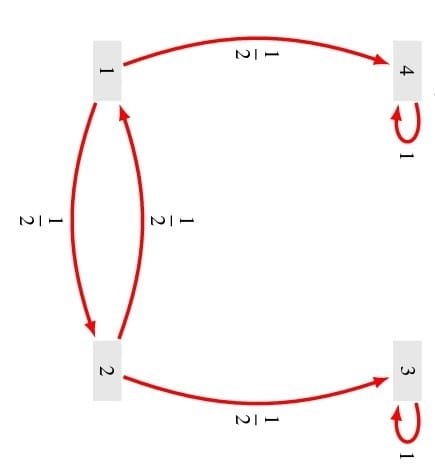
\includegraphics[width=\columnwidth,angle=90]{Theriotical Value.jpeg}
    \caption{Theriotical Results}
    \label{fig:Markov Chain}
\end{figure}
Here 1,2 states are transient and 3,4 states are absorbing. 
Let $\vec{P}$ denote the state transition matrix for the above markov chain.
\begin{align}\vec{P} =
\begin{bmatrix}
0 & 0.5 & 0 & 0.5 \\
0.5 & 0 & 0.5 & 0 \\
0 & 0 & 1 & 0 \\
0 & 0 & 0 & 1
\end{bmatrix}
\end{align}
\begin{lemma}


The standard form of the matrix is :
\begin{align}\vec{P} = 
\begin{bmatrix}
\vec{I} & \vec{O}\\
\vec{R} & \vec{Q} 
\end{bmatrix}
\end{align}
where $\vec{I},\vec{O}$ are Identity and Zero matrices and $\vec{R},\vec{Q}$ are other sub-matrices respectively.

\end{lemma}

After converting the transition matrix into the form of standard matrix we get
\begin{align} \vec{P} = 
\begin{bmatrix}
1 & 0 & 0 & 0 \\
0 & 1 & 0 & 0 \\
0 & 0.5 & 0 & 0.5 \\
0.5 & 0 & 0.5 & 0 
\end{bmatrix}
\end{align}
\begin{lemma}

The limiting matrix for absorbing markov chain is,
\begin{align}
\vec{P}= 
\begin{bmatrix}
\vec{I} & \vec{O} \\
\vec{FR} & \vec{O}
\end{bmatrix}
\end{align}

here $\vec{F}=\brak{\vec{I}-\vec{Q}}$ $^{-1}$ is called the fundamental matrix of $\vec{P}.$
\end{lemma}
Solving this leaves us with 
\begin{align}
\vec{P} = 
\begin{bmatrix}
1 & 0 & 0 & 0 \\
0 & 1 & 0 & 0 \\
0.333 & 0.667 & 0 & 0 \\
0.667 & 0.333 & 0 & 0
\end{bmatrix}
\end{align}
Here an element $\vec{P}_{ij}$ represents the probability of state j starting from state i. Let A be the event of getting the first head to appear on odd numberth trail starting with a odd numberth trail. Then the probability of A is   
\begin{align}
   \Pr(A) = p_{14} 
   & = 0.667
\end{align}
\end{document}
